\documentclass[11pt,letterpaper]{article}
\usepackage[top=3cm, bottom=2cm, left=2cm, right=2cm, columnsep=20pt]{geometry}
\usepackage{pdfpages}
\usepackage{graphicx}
\usepackage{etoolbox}
\apptocmd{\sloppy}{\hbadness 10000\relax}{}{}
% \usepackage[numbers]{natbib}
\usepackage[T1]{fontenc}
\usepackage{ragged2e}
\usepackage[french]{babel}
\usepackage{listings}
\usepackage{color}
\usepackage{soul}
\usepackage[utf8]{inputenc}
\usepackage[export]{adjustbox}
\usepackage{caption}
\usepackage{amsmath}
\usepackage{amssymb}
\usepackage{float}
\usepackage{csquotes}
\usepackage{fancyhdr}
\usepackage{wallpaper}
\usepackage{siunitx}
\usepackage[indent]{parskip}
\usepackage{textcomp}
\usepackage{gensymb}
\usepackage{multirow}
\usepackage[hidelinks]{hyperref}
\usepackage{abstract}
\renewcommand{\abstractnamefont}{\normalfont\bfseries}
\renewcommand{\abstracttextfont}{\normalfont\itshape}
\usepackage{titlesec}
\titleformat{\section}{\large\bfseries}{\thesection}{1em}{}
\titleformat{\subsection}{\normalsize\bfseries}{\thesubsection}{1em}{}
\titleformat{\subsubsection}{\normalsize\bfseries}{\thesubsubsection}{1em}{}

\usepackage{xcolor}
\definecolor{codegreen}{rgb}{0,0.6,0}
\definecolor{codegray}{rgb}{0.5,0.5,0.5}
\definecolor{codepurple}{rgb}{0.58,0,0.82}
\definecolor{backcolour}{rgb}{0.95,0.95,0.92}
\lstdefinestyle{mystyle}{
    backgroundcolor=\color{backcolour},   
    commentstyle=\color{codegreen},
    keywordstyle=\color{magenta},
    numberstyle=\tiny\color{codegray},
    stringstyle=\color{codepurple},
    basicstyle=\ttfamily\footnotesize,
    breakatwhitespace=false,         
    breaklines=true,                 
    captionpos=b,                    
    keepspaces=true,                 
    numbers=left,                    
    numbersep=5pt,                  
    showspaces=false,                
    showstringspaces=false,
    showtabs=false,                  
    tabsize=2
}
\lstset{style=mystyle}

\usepackage[most]{tcolorbox}
\newtcolorbox{note}[1][]{
  enhanced jigsaw,
  borderline west={2pt}{0pt}{black},
  sharp corners,
  boxrule=0pt, 
  fonttitle={\large\bfseries},
  coltitle={black},
  title={Note:\ },
  attach title to upper,
  #1
}

%----------------------------------------------------

\setlength{\parindent}{0pt}
\DeclareCaptionLabelFormat{mycaptionlabel}{#1 #2}
\captionsetup[figure]{labelsep=colon}
\captionsetup{labelformat=mycaptionlabel}
\captionsetup[figure]{name={Figure }}
\newcommand{\inlinecode}{\normalfont\texttt}
\usepackage{enumitem}
\setlist[itemize]{label=\textbullet}

\begin{document}
\begin{titlepage}
\center

\begin{figure}
    \ThisULCornerWallPaper{.4}{Polytechnique_signature-RGB-gauche_FR.png}
\end{figure}
\vspace*{2 cm}

\textsc{\Large \textbf{PHS2223 --} Introduction à l'optique moderne}\\[0.5cm]
\large{\textbf{Équipe : 04}}\\[1.5cm]

\rule{\linewidth}{0.5mm} \\[0.5cm]
\Large{\textbf{Expérience 3}} \\[0.2cm]
\text{Mesure de polarisation}\\
\rule{\linewidth}{0.2mm} \\[2.3cm]

\large{\textbf{Présenté à}\\
  Guillaume Sheehy\\
  Esmat Zamani\\[2.5cm]
  \textbf{Par :}\\
  Émile \textbf{Guertin-Picard} (2208363)\\
  Laura-Li \textbf{Gilbert} (2204234)\\
  Tom \textbf{Dessauvages} (2133573)\\[3cm]}

\large{\today\\
Département de Génie Physique\\
Polytechnique Montréal\\}

\end{titlepage}

%----------------------------------------------------

\tableofcontents
\pagenumbering{roman}
\newpage

\pagestyle{fancy}
\setlength{\headheight}{14pt}
\renewcommand{\headrulewidth}{0pt}
\fancyfoot[R]{\thepage}

\pagestyle{fancy}
\fancyhf{}
\renewcommand{\headrulewidth}{1pt}
\fancyhead[L]{\textbf{PHS2223}}
\fancyhead[C]{Rapport préliminaire}
\fancyhead[R]{\today}
\fancyfoot[R]{\thepage}

\pagenumbering{arabic}
\setcounter{page}{1}

%----------------------------------------------------

\section{Introduction}

Les ondes électromagnétiques ont plusieurs propriétés qui permettent d'expliquer les différents
phénomènes optiques observés dans la vie de tous les jours. L'une d'entre elles est la polarisation,
qui dicte la direction d'oscillation du champ électrique dans une onde électromagnétique. Elle
est fréquemment utilisée pour faire fonctionner différents objets communs, tels que des écrans à
cristaux liquides et des verres polarisés pour des lunettes. Ce laboratoire se concentre sur l'analyse
de cette propriété dans un système optique. Pour se faire, une expérience de mesure de puissance sera
faite avec des filtres polariseurs linéaires, qui permettent de ne laisser passer qu'une seule polarisation de
la lumière. Différents nombres et différentes orientations des polariesurs seront testés en laboratoire, mais
aussi modélisés mathématiquement au préalable. Ces modélisations seront faites à l'aide de deux formalismes, soit
le classique où l'expression standard d'une onde électromagnétique classique est utilisée, et le formalisme de
Jones, où l'état de polarisation d'une onde est décrit par un vecteur de Jones. Le document présent détaille
le fondement théorique de la polarisation et de ses formalismes, détaille les montages qui seront utilisés
pour l'expérience, et émet des hypothèses sur les observations à faire en laboratoire à l'aide du modèle
mathématique.

\section{Théorie}\label{theo}

yap yap

\subsection{Polarisation et polariseurs}

\subsection{Modèle classique}

\subsection{Modèle de Jones}



\section{Méthodologie}

yap yap

\subsection{Présentation des montages}

\subsection{Explications}



\section{Hypothèses}

Cette section utilise les deux modèles présentés à la section \ref{theo} pour simuler les mesures de
coefficients de transmission qui pourront être faits avec les montages.

\subsection{Modèle classique}

Avec le modèle classique, les courbes présentées à la figure \ref{classique} montrent la variation
du coefficient de transmission en fonction de la variation de l'angle $\theta$ autant pour le 
système à deux polariseurs qu'à trois polariseurs.

\begin{figure}[H]
  \centering
  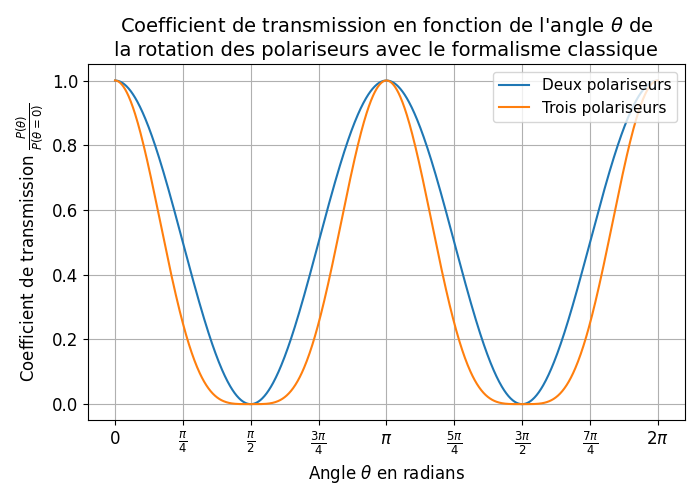
\includegraphics[scale=0.7]{coeff_classique.png}
  \caption{Coefficients de transmission pour le modèle classique.}
  \label{classique}
\end{figure}

Il est donc possible de faire comme hypothèse que le montage à deux polariseurs présente un comportement
sinusoidal entre 0 et 1 pour son coefficient de transmission. Quant au montage à trois polariseurs, cette
courbe est plus aplatie aux minimums et est toujours sous la courbe de deux polariseurs. La puissance est
donc réduite avec l'ajout du polariseur, mais les minimums de puissance restent aux mêmes angles.

\subsection{Modèle de Jones}

La figure \ref{jones} présente les mêmes courbes que pour le modèle classique, mais avec le modèle de Jones.

\begin{figure}[H]
  \centering
  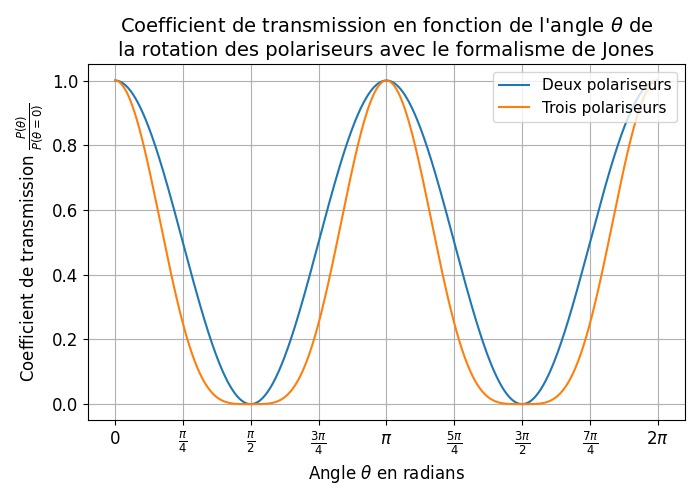
\includegraphics[scale=0.7]{coeff_jones.png}
  \caption{Coefficients de transmission pour le modèle de Jones.}
  \label{jones}
\end{figure}

Il est possible de voir que les résultats sont les mêmes que pour le modèle classique. Les hypothèses à émettre
sont donc les mêmes.


\clearpage

%\bibliographystyle{unsrtnat}
%\bibliography{camera_prelab.bib}

\end{document}
